\section{Introduction}

% 城市客流预测是智能交通系统的基础支撑，服务于交通调度、运力配置、拥堵缓解与公共安全管理。在传感器、共享出行与移动设备数据不断积累的推动下，深度序列与时空模型在刻画日周期、周周期以及局部空间依赖上取得了显著进展。然而这些模型隐含假设未来客流会延续充足历史中观察到的常规模式；一旦城市偏离常规运行状态，仅依赖这些模式的预测就难以满足实际需求。

Urban flow forecasting underpins modern intelligent transportation systems, providing essential support for traffic scheduling, capacity allocation, congestion mitigation, and public safety management. Driven by the continual accumulation of sensor, ride-sharing, and mobile-device data, deep sequential and spatiotemporal models have made remarkable progress in characterizing both daily and weekly periodicity as well as local spatial dependencies~\cite{lstm,dlinear,PatchTST,timesnet,moderntcn}. Such models, however, implicitly assume that future flows will continue the regular patterns observed throughout an abundant history. Once a city departs from its regular operating state, forecasts built solely on these patterns quickly fall short of practical requirements.

\begin{figure}[t]
   \centering
    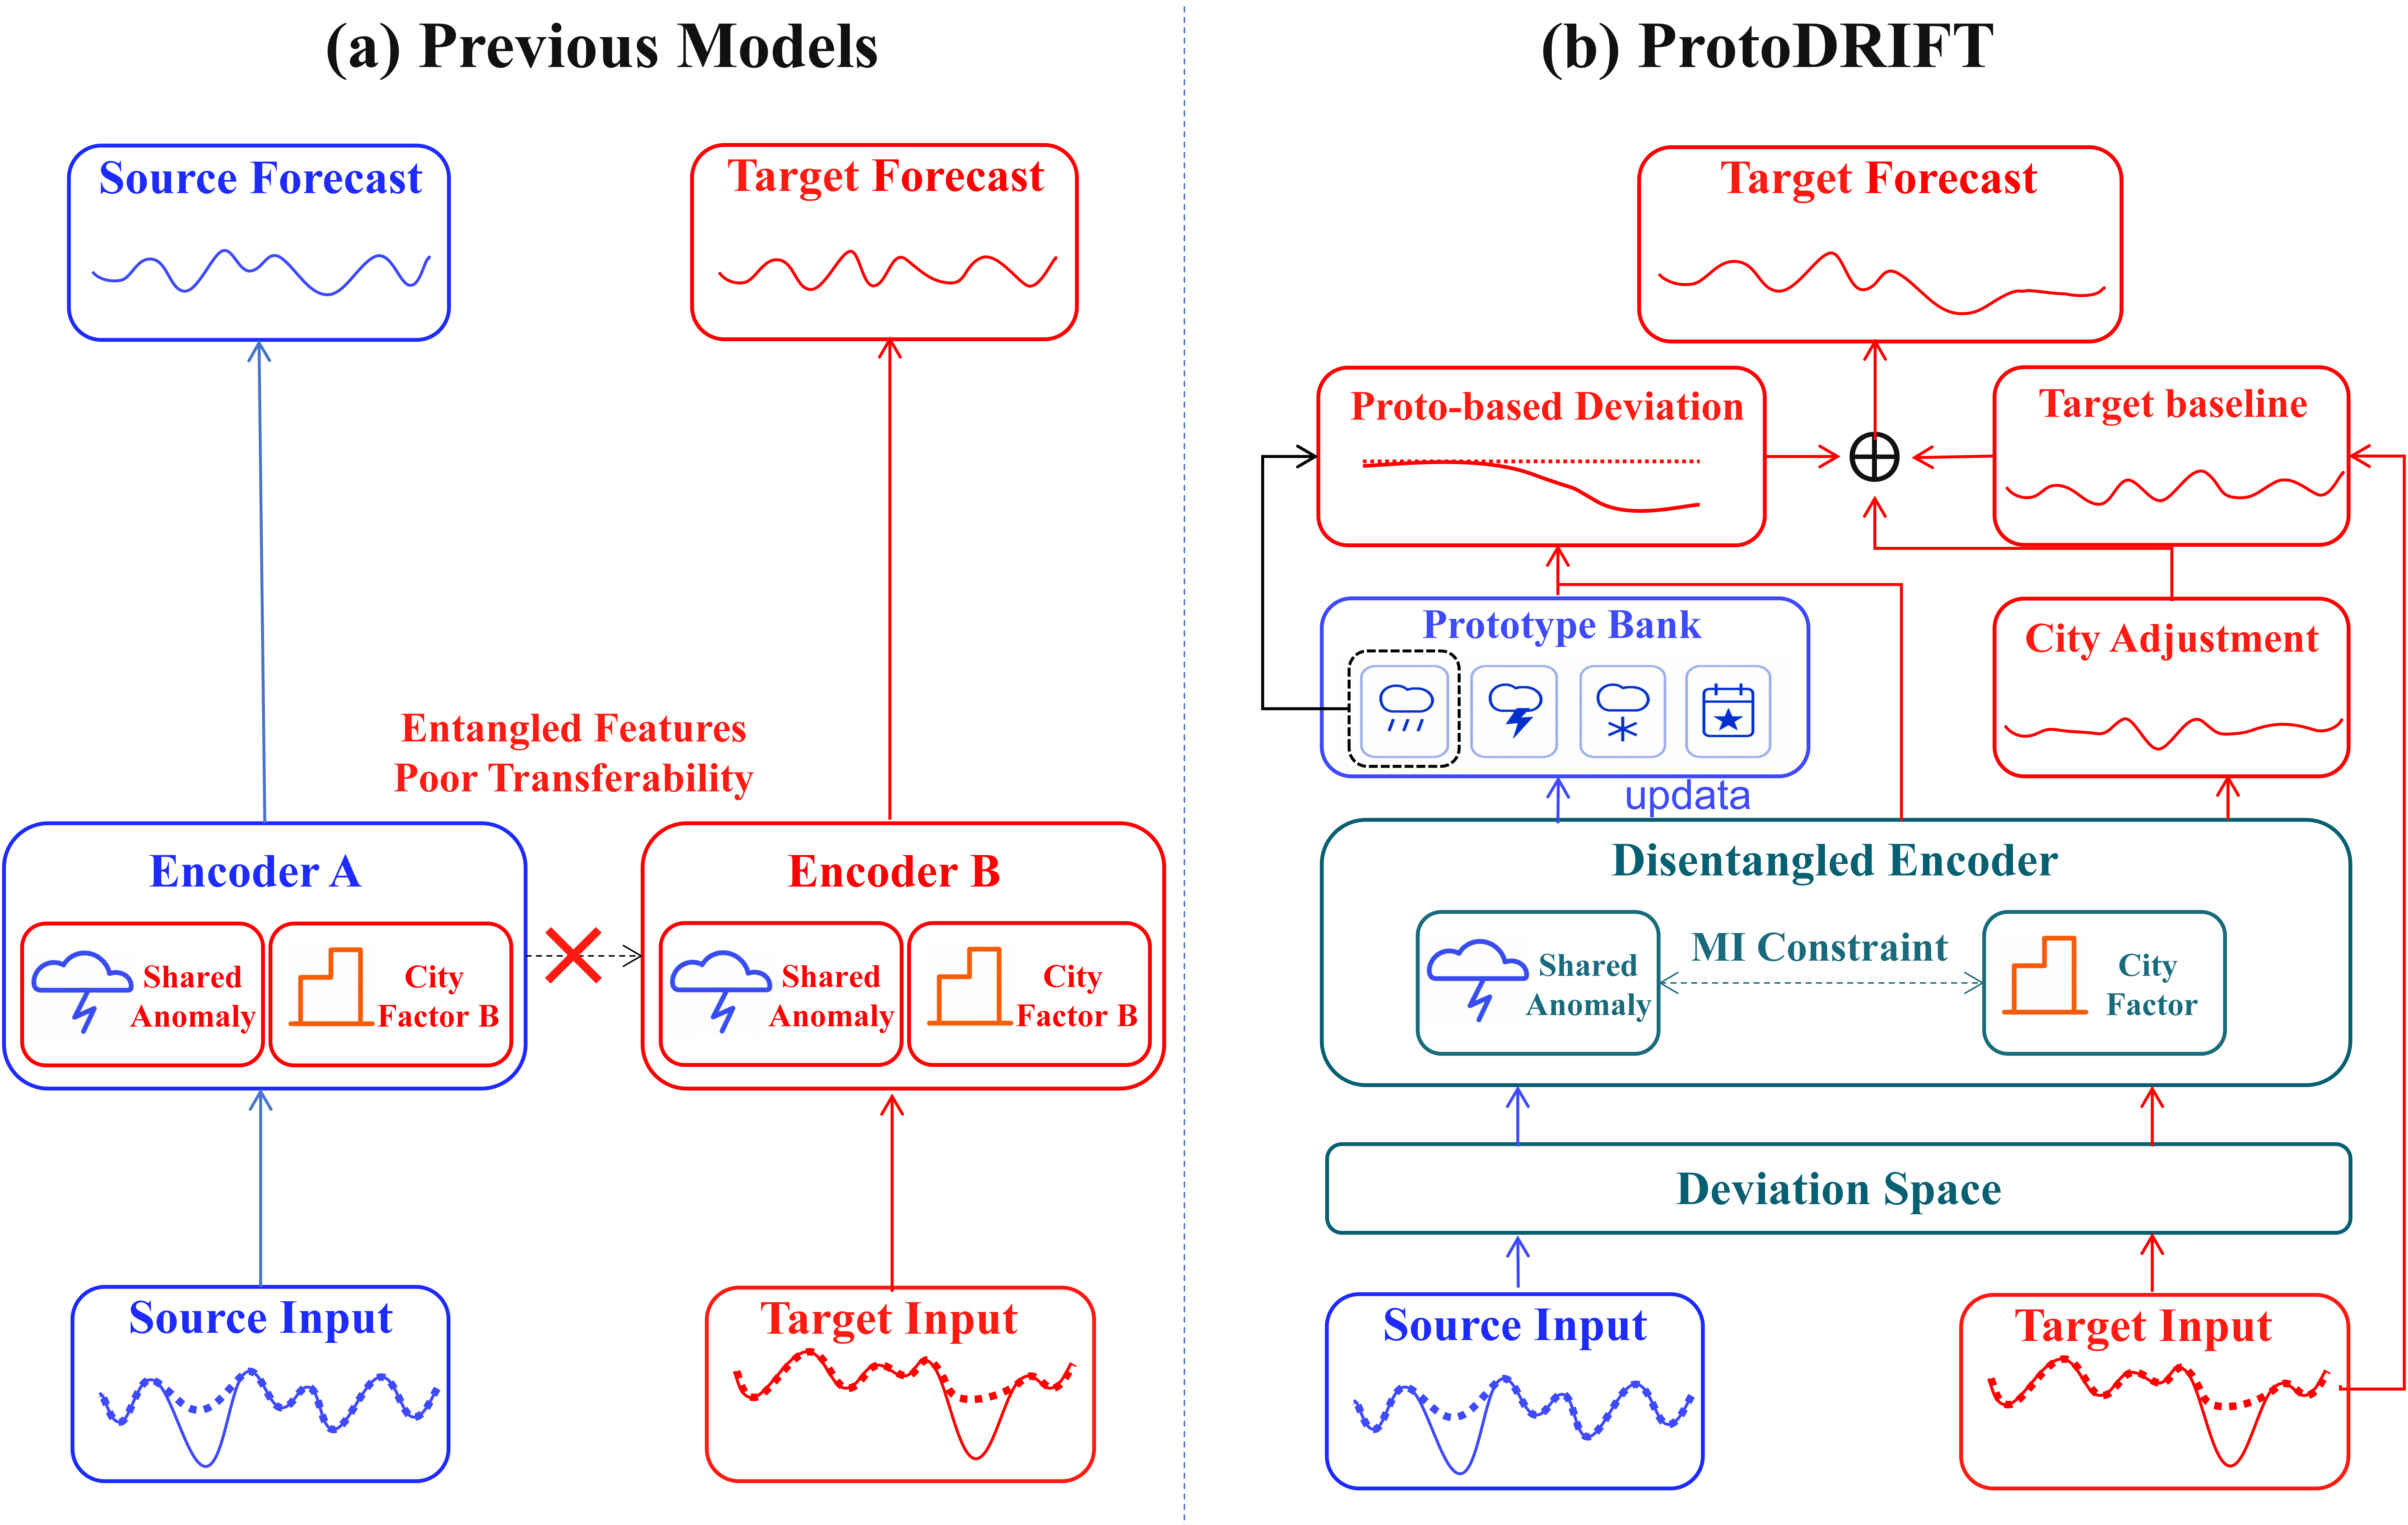
\includegraphics[width=0.50\textwidth]{fig/introduction_01.png} % Reduce the figure size so that it is slightly narrower than the column.
    \caption{Illustration of cross-city anomalous urban flow forecasting. (a) Existing models entangle the shared anomaly response with city-specific factors, so the source-city encoder cannot be reused. (b) ProtoDRIFT instead learns anomaly semantics in the deviation space, where a prototype bank makes them reusable across cities and a city-conditioned branch recalibrates only the target-city magnitude.}
    \label{fig:intro}
\end{figure}

% 已有超越该假设的努力大致分为两条路线。第一条追求分布漂移下的通用鲁棒性：实例归一化、分布对齐与混杂因素感知设计缓解训练与测试时段之间的统计量变化，更强的骨干网络则扩展了长序列与多周期序列的建模能力。第二条则显式针对稀有的高影响观测：极值启发的损失、不平衡感知目标以及原型或记忆增强结构提升了极值与异常时段的精度，并有事故对齐、上下文丰富的移动性数据集作为支撑。但这两条路线都在单一域内训练与评测，且仍在绝对客流空间中直接回归。

Existing efforts to move beyond this assumption can be broadly grouped into two complementary lines. The first pursues general robustness under distribution shifts, where instance normalization, distribution alignment, and confounder-aware designs mitigate the shifting statistics observed between training and test periods~\cite{revin,timealign,steve}, while progressively stronger backbones enlarge the modeling capacity for long and multi-periodic sequences~\cite{iTransformer,autoformer,informer,crossformer}. The second line instead explicitly targets rare, high-impact observations, where extreme-value-inspired losses, imbalance-aware objectives, and prototype- or memory-augmented structures improve accuracy on extreme values and anomalous periods~\cite{evl,ealgap,dan,stssdl}, supported by benchmarks that supply incident-aligned and context-rich mobility data~\cite{traffident,stcontext}. Both lines, however, are typically trained and evaluated within a single domain and still regress the flows themselves directly in the absolute-value space.

% 异常观测在城市间的分布不均使可迁移的异常建模变得必要：单个城市很少能积累足够的节假日或极端天气事件，而不同城市却可能共享这类事件所引发的响应模式。如图 1(a) 所示，已有模型把共享的异常响应与城市特有因素——客流量级、局部空间结构与周期性习惯——编码进同一个纠缠表示，因此源城市上学到的编码器无法在目标城市复用。由此带来两个困难。其一，异常样本稀缺且与正常客流差异显著，在大量正常样本上拟合的模型容易低估异常偏移，或把它吸收进城市特有的基线中。其二，同类事件在不同城市的发生频率、强度、空间覆盖与持续时间各不相同，使得在原始客流空间中对齐并不可靠；对齐边缘分布或直接复用源城市原型甚至可能引入系统性偏差。

The uneven availability of anomalous observations across cities makes transferable anomaly modeling not merely desirable but essential: a single city rarely accumulates a sufficient number of holiday or extreme-weather episodes, whereas different cities plausibly share the response patterns that such events induce. As illustrated in Figure~\ref{fig:intro}(a), existing models encode the shared anomaly response together with city-specific factors—flow magnitude, local spatial structure, and periodic habits—inside one entangled representation, so the encoder learned on a source city can hardly be reused on a target city. Two concrete difficulties follow from this entanglement. First, anomalous samples are scarce and deviate markedly from normal flows, so a model fitted on abundant normal samples tends to underestimate anomalous shifts or absorb them into the city-specific baseline. Second, the same event type differs across cities in frequency, intensity, spatial coverage, and duration, which makes alignment in the raw flow space unreliable; aligning marginal distributions or directly reusing source-city prototypes may even introduce systematic bias~\cite{timealign,protots}.

% 分解式预测提示了一条出路：把序列拆成性质不同的分量——季节与趋势、周期与残差，或图层面的因子——所得到的分量比原始信号泛化得更好。我们的核心观察是，城市客流同样可以拆分为城市特有的正常基线和相对更可迁移的异常偏差。与直接迁移尺度差异显著的绝对值不同，我们先用正常基线刻画目标城市自身的常规节律，再在相对该基线的偏差空间中学习异常动态。基于这一洞见，我们提出如图 1(b) 所示的 ProtoDRIFT。在偏差空间中运作的解耦编码器把每个窗口拆为共享异常表示与城市因子，互信息约束抑制二者之间的冗余依赖。共享表示查询一个紧凑的原型库以归纳反复出现的偏差形态，产生基本不依赖城市尺度的原型偏差；城市条件分支随后恢复目标城市的量级与局部响应，最终预测由该调整后的偏差与目标城市基线重组而成。

Decomposition-based forecasting suggests a promising way out of this dilemma: splitting a series into components of different natures—seasonal and trend, periodic and residual, or graph-level factors—yields parts that each generalize far better than the raw signal does~\cite{cost,hyperd,tgdl}. Our key observation is that urban flows naturally admit an analogous split into a city-specific normal baseline and relatively more transferable anomaly deviations. Rather than transferring absolute values whose scales differ substantially across cities, we first characterize the target city's own regular rhythm with a normal baseline and learn anomalous dynamics in the deviation space relative to it. Leveraging this insight, we accordingly develop \textbf{ProtoDRIFT}, shown in Figure~\ref{fig:intro}(b). A disentangled encoder operating in the deviation space splits each window into a shared anomaly representation and a city factor, and a mutual-information constraint suppresses the redundant dependence between them. The shared representation queries a compact prototype bank that summarizes recurring deviation shapes, yielding a prototype-based deviation that is largely independent of city scale; a separate city-conditioned branch then restores the magnitude and local response of the target city, and the final forecast recomposes this adjusted deviation with the target-city baseline.

% 本文的主要贡献有三点：
% 1. 概念洞见。我们指出城市特有尺度与可迁移异常语义的纠缠是跨城市异常客流预测的核心障碍，并在“城市特有正常基线 + 可迁移异常偏差”的视角下将该任务重构为偏差参照的迁移问题。
% 2. 方法框架。我们提出 ProtoDRIFT，在偏差空间中学习紧凑的异常偏差原型库，并通过互信息约束与城市条件调整分支，将可迁移的异常语义与城市条件响应相分离。
% 3. 实验验证。我们在 NYC 与 CHI 之间的双向零样本迁移设定下开展系统实验，同时评估 full 与 anomaly 子集，并通过主实验对比、消融研究、设计变量敏感性与可解释性分析验证所提设计。

Our main contributions are threefold:

\begin{itemize}
    \item \textbf{Conceptual insight.} We identify the entanglement of city-specific scales and transferable anomaly semantics as the core obstacle to cross-city anomalous flow forecasting, and accordingly reformulate the task as a deviation-referenced transfer problem under the unified perspective of "city-specific normal baseline + transferable anomaly deviation".
    \item \textbf{Methodological framework.} We present ProtoDRIFT, which learns a compact bank of anomaly deviation prototypes directly in the deviation space and explicitly separates transferable anomaly semantics from city-conditioned responses via a mutual-information constraint together with a city-conditioned adjustment branch.
    \item \textbf{Empirical validation.} We conduct systematic experiments under bidirectional zero-shot transfer between NYC and CHI, evaluating both the full and anomaly subsets, and verify the effectiveness of the proposed designs through main comparisons, ablation studies, design-variable sensitivity, and interpretability analyses.
\end{itemize}
